%%Chapter - Split into separate file if too large
\chapter{Dips and Extras}
%% Start recipe
\newrecipe{Tomato Tapenade}{http://www.taste.com.au/recipes/10128/sun+dried+tomato+tapenade}

\section*{Ingredients}
\begin{ingredients-list}
	\item 110g (1 cup) drained sun-dried tomatoes
	\item 2 garlic cloves, peeled
	\item \sfrac{1}{2} cup firmly packed fresh basil leaves, washed, dried well
	\item 3 anchovy fillets, drained
	\item 3\sfrac{1}{2} tbs extra virgin olive oil
	\item 1\sfrac{1}{2} tsp Worcestershire sauce 
\end{ingredients-list}

\section*{Directions}
\begin{enumerate}
\item Combine sun-dried tomatoes, garlic cloves, basil leaves and anchovy fillets in the bowl of a food processor and process until roughly chopped.
\item Add 3 tbs of the extra virgin olive oil and Worcestershire sauce and process until smooth and well combined.
\item Spoon mixture into hot sterilized jars, cover surface of tapenade with the remaining extra virgin olive oil and seal immediately. Store in the fridge for up to 3 months.
\end{enumerate}
%%End Recipe

%%Begin recipe
\newrecipe{Hummus}{http://www.taste.com.au/recipes/5103/hummus}
%\begin{figure}[h!]
%\centering
%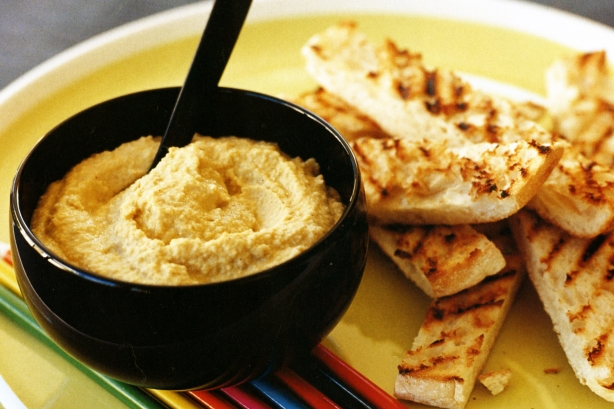
\includegraphics[scale=0.5]{img/hummus.jpg}
%\end{figure}
\bigskip
\section*{Ingredients}
\begin{ingredients-list}
	\item 600g canned chickpeas, drained, rinsed
		\begin{textblock*}{8cm}(8.5cm,-1.2cm) % {block width} (coords)
			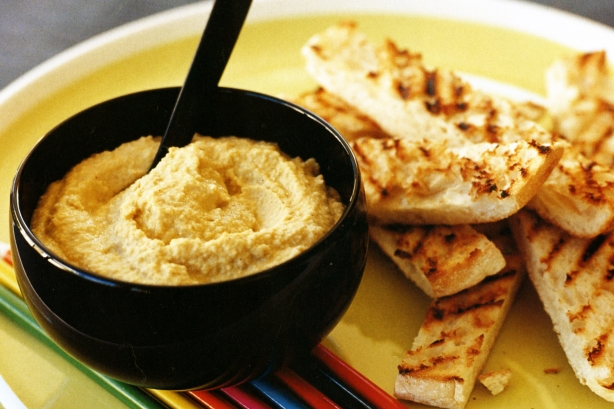
\includegraphics[scale=0.35]{./img/hummus.jpg}
		\end{textblock*}
	\item 3 garlic cloves, crushed
	\item 100ml olive oil
	\item 2 tbs tahini paste*
	\item 1 tsp ground cumin
	\item Juice of 1 lemon
	\item Toasted Turkish bread, to serve
\end{ingredients-list}

\section*{Directions}
\begin{enumerate}
	\item Place the chickpeas, garlic, olive oil, tahini paste, cumin and lemon juice in a food processor and process until combined.
		Add 1/4 cup (60ml) of water and process again until quite smooth.
	\item Place hummus in a bowl and serve with toasted Turkish bread.
\end{enumerate}
%%End recipe

%%Begin recipe
\newrecipe{Tomato Kasundi}{http://www.taste.com.au/recipes/6482/tomato+kasundi}
\label{tomato_kasundi}
\hypertarget{tomato_kasundi}{}%target for hyperlink from recipes using this recipe.
\section*{Ingredients}
\begin{ingredients-list}
	\item 60ml sunflower oil
	\item 1 tablespoon black mustard seeds
	\item 1 tablespoon turmeric
	\item 2 tablespoons cumin
	\item 2 teaspoons chilli powder
	\item \sfrac{1}{4} cup peeled, grated fresh ginger
	\item 4 crushed garlic cloves
	\item 1 seeded, finely chopped green chilli
	\item 30ml of malt vinegar
	\item 2x 400g cans diced tomatoes
	\item \sfrac{1}{3} cup brown sugar
	\item 1 teaspoon salt
	\item 130ml malt vinegar
\end{ingredients-list}

\section*{Directions}
\begin{enumerate}
	\item Heat 60ml sunflower oil in a large saucepan until hot.
		Add 1 tablespoon black mustard seeds,1 tablespoon turmeric, 2 tablespoons cumin and 2 teaspoons chilli powder.
		Cook, stirring, for 5 minutes to release the flavours.
	\item Add \sfrac{1}{4} cup peeled, grated fresh ginger, 4 crushed garlic cloves, 1 seeded, finely chopped green chilli and 30ml of malt vinegar and cook for 5 minutes.
	\item Add two 400g cans diced tomatoes, \sfrac{1}{3} cup brown sugar, 1 teaspoon salt and 130ml malt vinegar and simmer for 1-1\sfrac{1}{2} hours.
	\item The kasundi is ready when the oil comes to the top.
\end{enumerate}
%%End recipe

%%Begin recipe
\newrecipe{Caramelised Onion}{http://www.jilldupleix.com/recipes/rec052.php}
\label{caramelised_onion}
\hypertarget{caramelised_onion}{}%target for hyperlink from recipes using this recipe.

\section*{Ingredients}
\begin{ingredients-list}
\item 1 kg red (or brown) onions, peeled
\item 1 tsp. sea salt
\item \sfrac{1}{2} tsp. freshly ground black pepper
\item 2 bay leaves
\item 2 rosemary sprigs
\item 100 ml olive oil
\item 150 g soft brown sugar
\item 100 ml dry white wine
\item 75 ml red wine vinegar (Use balsamic vinegar instead)
\end{ingredients-list}

\section*{Directions}
\begin{enumerate}
\item Cut the onions in half and slice finely ( a boring task, but think of all the pleasure ahead).
	In a heavy fry pan, toss the onion in the olive oil. Cook over gentle heat until the onions start to colour.
	Add the salt, pepper, bay leaves and rosemary sprigs, cover and cook over gentle heat for 20 minutes until soft and wilted.
\item Remove the lid and add the sugar, wine and vinegar.
	Bring to the boil, stirring, then reduce the heat and cook, uncovered, for a further 20 to 30 minutes until the liquid has been absorbed by the onions, and they are soft and sticky.
	You'll need to stir fairly constantly towards the end of cooking time to avoid scorching.
\item Pick out the bay leaves and rosemary and discard. Spoon the relish into a clean, dry, sterilised jar, leave to cool, then seal tightly. Will keep in the fridge for 2 weeks.
\end{enumerate}
%%End Recipe
